\documentclass[10pt, red]{beamer}
\usetheme{JuanLesPins}
\usepackage[english]{babel}
\usepackage[latin1]{inputenc} 
\setbeamercovered{transparent}


\title[CUDAQCADesigner]{A Parallel Version of the MiNa's Quantum Dot Cellular Automata IDE - QCADesigner}

\author{Riccardo Cattaneo, Giuseppe Chindemi}

\institute{
  Politecnico di Milano\\
  HPPS
}

\date{June 22 2010}

\pgfdeclareimage[height=0.5cm]{logo}{img/polimi}
\logo{\pgfuseimage{logo}}


\begin{document}

\begin{frame}
  \titlepage
\end{frame}

\section{Introduction}
	\begin{frame}{Why?}
		\begin{itemize} 
			\item Si based technology is reaching its physical limits due to aggressive miniaturization, progressively increasing packaging densities, clock distribution and dissipation issues
			\item Alternatives are being studied right now in order to overcome these limits (different technologies)
			\item QCA cells are one of these
			\item QCADesigner is the most mature tool for layouting and simulating QCA cells based circuits, yet, in the original implementation it is unreasonably slow to simulate more bigger-than-toy ones
			\item Exploitation of CUDA in order to obtain significant speedups
		\end{itemize}
	\end{frame}

\section{QCA cells}
	\begin{frame}{QCA cells? Why?}
		\begin{columns}
		\centering
	
    		\column{.49\textwidth}
			Limits of current transistor technology 
		 	\begin{itemize}
			 	\item	\textbf{Shrinking size} in practice: no less than $  20 \mu m $ (nowadays: $45\mu m$)
			 	\item \textbf{Reduced clock frequency} in practice: in the order of magnitude of $10^9 Hz$
			 	\item \textbf{Power dissipation problem}
		 	\end{itemize}
			 	
			\column{.49\textwidth}
			QCA cells technology
		 	\begin{itemize}
			 	\item \textbf{Improved clock frequency} in practice: in the order of magnitude of $10^{12} Hz$
			 	\item \textbf{Power dissipation} in practice: in the order of magnitude of $10^{-18} W$
			 	\item \textbf{Device density} in practice: in the order of magnitude of $10^{10} W$
		 	\end{itemize}
		\end{columns}
	\end{frame}



	\begin{frame}{QCA cells? What?}
		\begin{columns}
    		\column{.5\textwidth}
		 	\begin{figure}
				\centering
				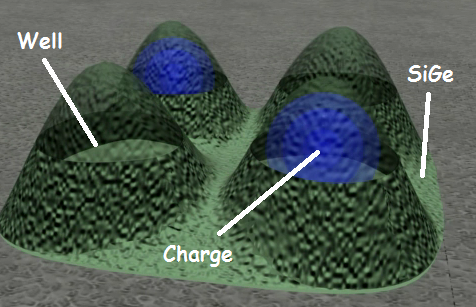
\includegraphics[width=\textwidth]{img/qca.png}
				\caption{QCA cells: physical view.}
		 	\end{figure} 
			\column{.5\textwidth}
			\begin{figure}
				\centering
				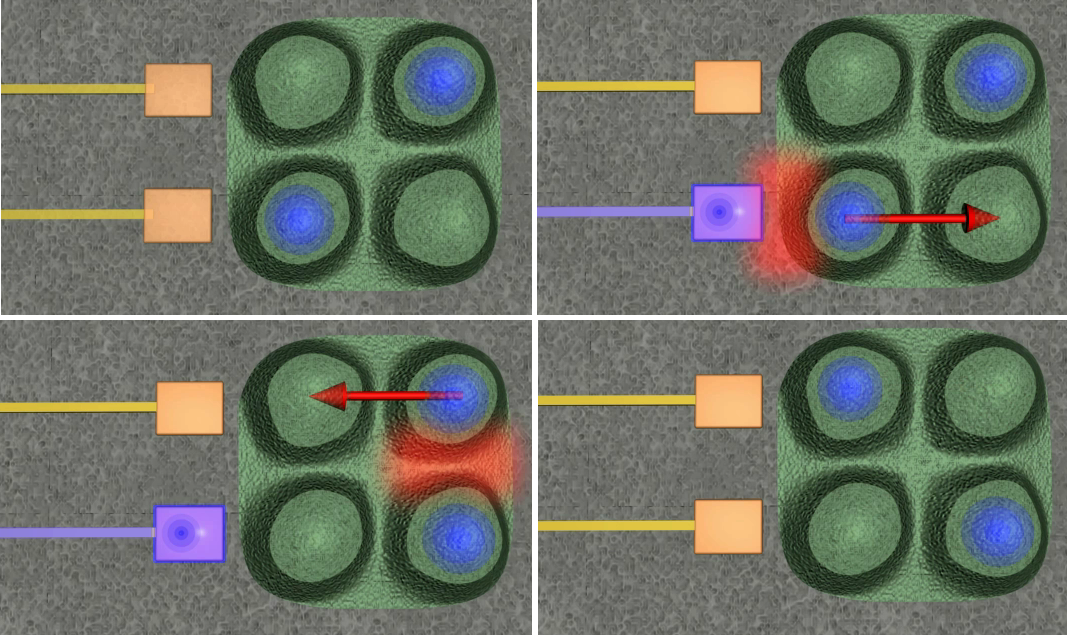
\includegraphics[width=\textwidth]{img/qcaevo.png}
				\caption{QCA cells: evolution of local state.}
			\end{figure}
		\end{columns}
		QCA are CA: evolution depends on previous status of cell itself and neighborhood
	\end{frame}


\section{Nvidia CUDA}

	\begin{frame}{CUDA Overview}
		What is CUDA?		
		\begin{itemize}
			\item It is a software layer that allow programmers to exploit the capability of Nvidia GPUs as general purpose processors.
		\end{itemize}
		Why CUDA for QCAD?
		\begin{itemize}
			\item Because QCA are parrallel by nature.
			\item Because GPUs are good in arithmeric.
			\item Because GPUs offer the lowest price per core.
		\end{itemize}
	\end{frame}

	\begin{frame}{GPU Logical Organization and Programming Model}
		\begin{columns}
    		\column{.4\textwidth}
		 	\begin{figure}
				\centering
				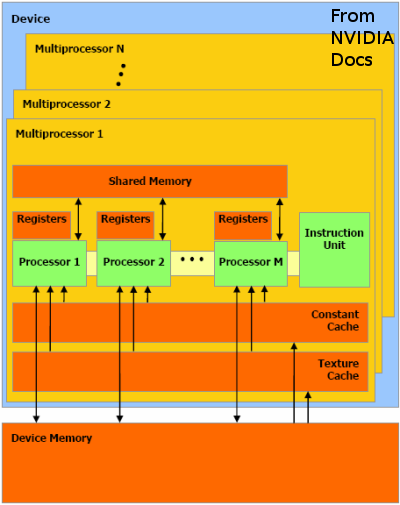
\includegraphics[width=\textwidth, height=0.6\textheight]{img/HWModel}
				\caption{CUDA GPUs: A MIMD Array of SIMD processors}
		 	\end{figure} 
			\column{.4\textwidth}
			\begin{figure}
				\centering
				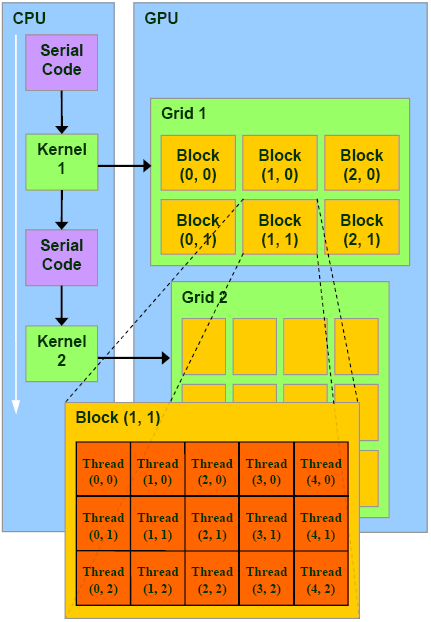
\includegraphics[width=\textwidth, height=0.6\textheight]{img/nVidiaExecutionModel}
				\caption{CUDA GPUs: Heterogeneous Programming}
			\end{figure}
		\end{columns}
	\end{frame}


\section{Implementation}
	\begin{frame}{Original Implementation}
		\begin{itemize}
			\item Every cell-one thread approach
			\item Additive error when evolving system
			\item Time complexity: $O(2^i*n*b)$
		\end{itemize}
		Every cell is simulated one after the other even though they could be evolved in parallel
	\end{frame}

	\begin{frame}{CUDA Implementation}
		\begin{itemize}
			\item One cell-one thread approach
			\item No additive error when evolving system
			\item Time complexity: $(\frac{2^i*n*b}{T})$ where $T$ is the number of running threads
		\end{itemize}
		Every thread is responsible for the evolution of its cell. The larger the number of running threads, the better the performances (upper bound: $T$=number of cells in the layout)
	\end{frame}

\section{Results}

	\begin{frame}{Tests Description}
		The "Lucifero" Workstation
		\begin{description}
			\item[CPU] Intel Xeon E5345
			\item[GPU] Nvidia Testa C1060
		\end{description}
		Which Tests?
		\begin{description}
			\item[Test 1] QCAD vs CUDAQCAD
			\item[Test 2] Memory Transfert Rate
			\item[Test 3] GPU Occupancy
		\end{description}
	\end{frame}

	\begin{frame}{Test 1: QCAD vs CUDAQCAD}
	 	\begin{figure}
			\centering
			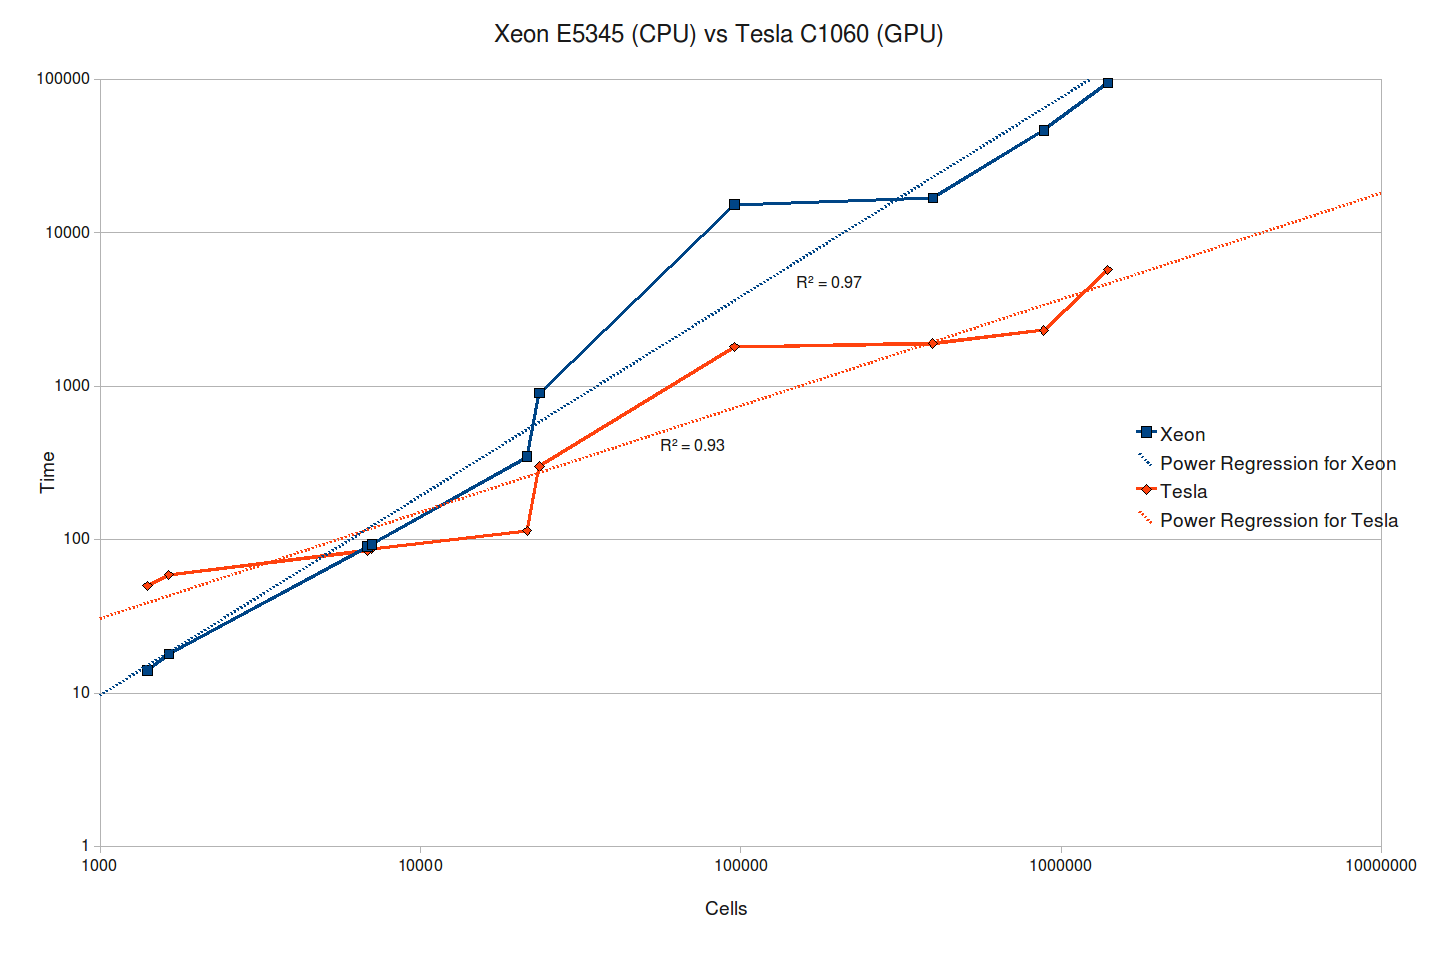
\includegraphics[width=\textwidth]{img/xeonvstesla}
	 	\end{figure} 
	\end{frame}

	\begin{frame}{Test 1: QCAD vs CUDAQCAD}
	 	\begin{figure}
			\centering
			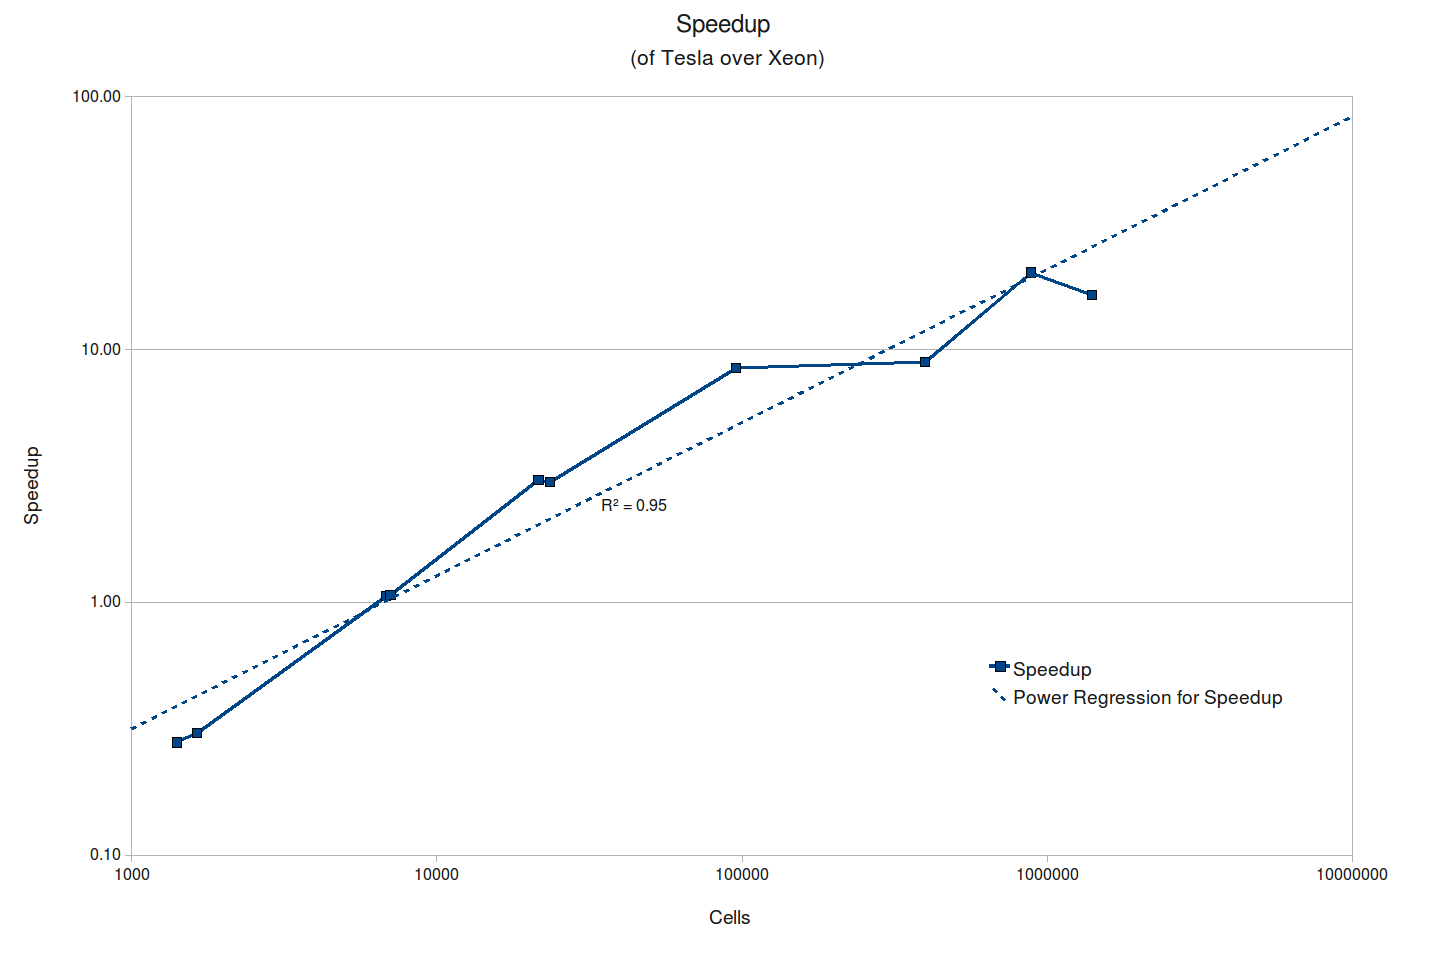
\includegraphics[width=\textwidth]{img/speedup}
	 	\end{figure} 
	\end{frame}

	\begin{frame}{Test 2: Memory Transfert Rate}
	 	\begin{figure}
			\centering
			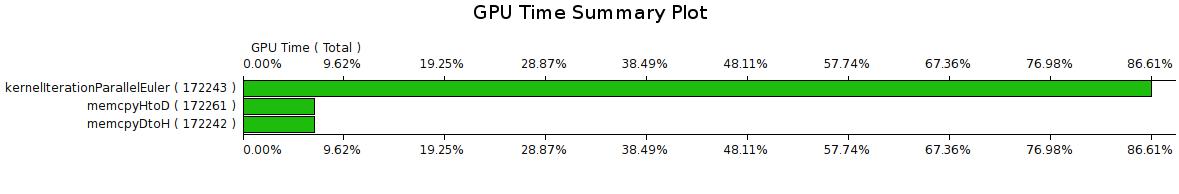
\includegraphics[width=\textwidth]{img/GPUTimeSummaryPlotNAND}
			\caption{Memory Tranfer for NAND circuit (1642 cells)}
	 	\end{figure} 
		\begin{figure}
			\centering
			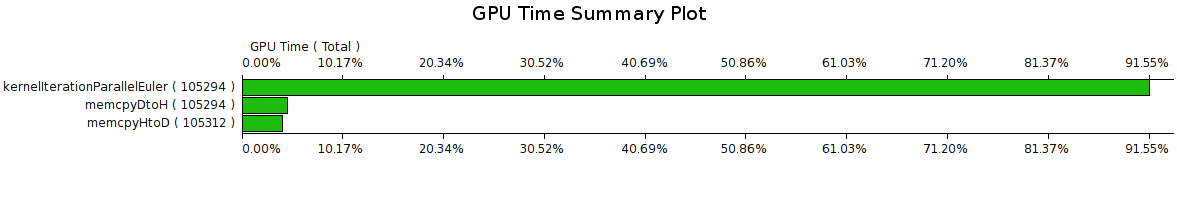
\includegraphics[width=\textwidth]{img/GPUTimeSummaryPlotMUX42}
			\caption{Memory transfers for MUX42 circuit (21551 cells)}
		\end{figure}
	\end{frame}

	\begin{frame}{Test 3: GPU Occupancy}
	 	\begin{figure}
			\centering
			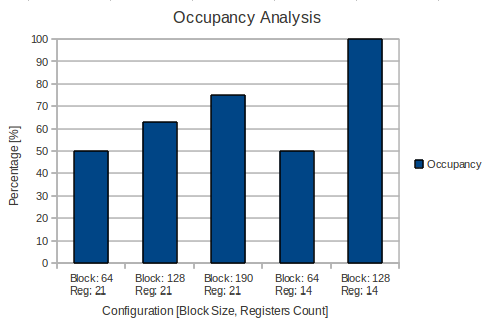
\includegraphics[width=\textwidth]{img/OccupancyAnalysis}
	 	\end{figure} 
	\end{frame}

	\begin{frame}{Questions?}
		\begin{columns}
		\column{.2\textwidth} 
			\textbf{Questions?}
		\end{columns}
	\end{frame}


\end{document}
